\pgfplotsset{width=.98\linewidth, height=4.7cm}
\begin{minipage}[h]{.49\linewidth}
	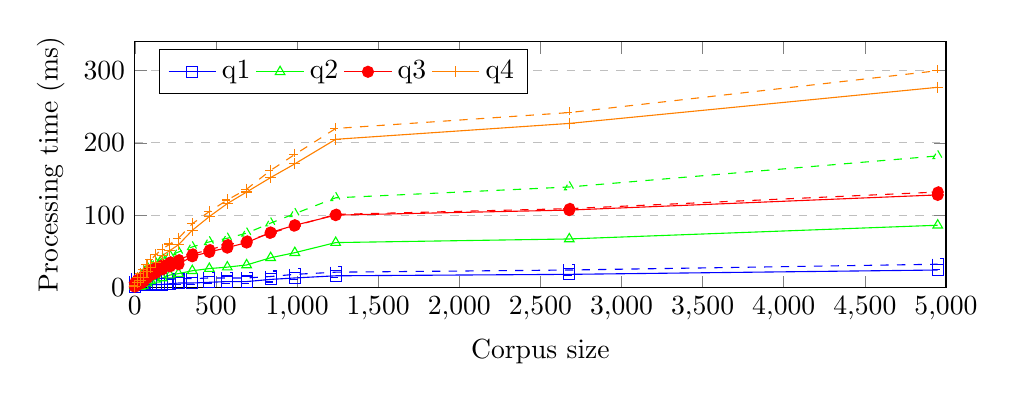
\begin{tikzpicture}[scale=1]
	\begin{axis}[
	xlabel={Corpus size},
	ylabel={Processing time (ms)},
	xmin=0, xmax=5000,
	ymin=0, ymax=340,
	legend pos=north west,
	ymajorgrids=true,
	grid style=dashed,
	legend style={legend columns=4},
	%ymode=log,
	%xmode=log,
	]
	
	    \addplot[
        color=blue,
        mark=square,
        samples=100
        ]
        coordinates {
(0,1)
(16,4)
(33,4)
(53,4)
(75,4)
(97,4)
(128,4)
(169,4)
(216,5)
(269,6)
(354,6)
(459,7)
(570,8)
(689,8)
(837,11)
(986,13)
(1238,16)
(2678,18)
(4949,24)
 };
    \addplot[
color=blue,
mark=square,
dashed,
samples=100
]
coordinates {
	(0,8)
	(16,12)
	(33,11)
	(53,11)
	(75,11)
	(97,11)
	(128,11)
	(169,11)
	(216,11)
	(269,12)
	(354,12)
	(459,13)
	(570,13)
	(689,13)
	(837,15)
	(986,18)
	(1238,21)
	(2678,24)
	(4949,32)
};

\addplot[
        color=green,
        mark=triangle,
        ]
        coordinates {
(0,1)
(16,1)
(33,1)
(53,2)
(75,6)
(97,9)
(128,11)
(169,13)
(216,17)
(269,19)
(354,23)
(459,26)
(570,28)
(689,31)
(837,41)
(986,48)
(1238,62)
(2678,67)
(4949,86)
        };
\addplot[
color=green,
dashed,
mark=triangle,
]
coordinates {
	(0,7)
	(16,13)
	(33,16)
	(53,21)
	(75,27)
	(97,31)
	(128,34)
	(169,40)
	(216,44)
	(269,49)
	(354,56)
	(459,63)
	(570,68)
	(689,75)
	(837,89)
	(986,102)
	(1238,124)
	(2678,139)
	(4949,182)
};

\addplot[
        color=red,
        mark=*,
        ]
        coordinates {
(0,1)
(16,4)
(33,5)
(53,8)
(75,13)
(97,17)
(128,20)
(169,25)
(216,29)
(269,32)
(354,43)
(459,49)
(570,55)
(689,62)
(837,76)
(986,86)
(1238,100)
(2678,107)
(4949,128)
        };
\addplot[
color=red,
dashed,
mark=*,
]
coordinates {
	(0,7)
	(16,11)
	(33,12)
	(53,16)
	(75,21)
	(97,24)
	(128,27)
	(169,31)
	(216,35)
	(269,38)
	(354,46)
	(459,52)
	(570,59)
	(689,64)
	(837,75)
	(986,85)
	(1238,101)
	(2678,109)
	(4949,132)
};

\addplot[
        color=orange,
        mark=+,
        ]
        coordinates {
(0,1)
(16,7)
(33,9)
(53,14)
(75,22)
(97,27)
(128,34)
(169,44)
(216,51)
(269,59)
(354,79)
(459,98)
(570,116)
(689,132)
(837,152)
(986,171)
(1238,205)
(2678,227)
(4949,277)
        };
\addplot[
color=orange,
mark=+,
dashed
]
coordinates {
	(0,3)
	(16,14)
	(33,19)
	(53,25)
	(75,32)
	(97,38)
	(128,45)
	(169,53)
	(216,60)
	(269,68)
	(354,88)
	(459,105)
	(570,121)
	(689,136)
	(837,162)
	(986,184)
	(1238,220)
	(2678,242)
	(4949,300)
};

	
	\legend{q1, , q2, , q3, , q4, }
	\end{axis}
	\end{tikzpicture}
		\vspace*{-.75cm}
	\caption{\label{fig:executionTime} Execution time with and without synonyms}
\end{minipage}